% DreamLab AI-Powered Knowledge Work Programme - B2B Sales Pitch
\documentclass[aspectratio=169,12pt]{beamer}
\usetheme{metropolis}
\usepackage{appendixnumberbeamer}
\usepackage{booktabs}
\usepackage{tikz}
\usepackage{pgfplots}
\usepackage{eurosym}
\usepackage{fontawesome5}
\usepackage{graphicx}
\usepackage{array}
\usepackage{xcolor}

% Colour scheme
\definecolor{dreamblue}{RGB}{0,123,255}
\definecolor{dreamgreen}{RGB}{0,204,153}
\definecolor{dreamgrey}{RGB}{102,102,102}
\definecolor{dreamdark}{RGB}{33,33,33}
\definecolor{warningred}{RGB}{255,99,71}

\setbeamercolor{frametitle}{bg=dreamblue}
\setbeamercolor{progress bar}{fg=dreamgreen}
\setbeamercolor{alerted text}{fg=dreamgreen}

% Custom commands
\newcommand{\highlight}[1]{\textcolor{dreamgreen}{\textbf{#1}}}
\newcommand{\pain}[1]{\textcolor{warningred}{\textbf{#1}}}
\newcommand{\benefit}[1]{\textcolor{dreamgreen}{\faCheckCircle{} #1}}
\newcommand{\note}[1]{\textit{\small Note: #1}}

\title{Transform Your Council's Productivity}
\subtitle{AI-Powered Knowledge Work Programme}
\date{June 2025}
\author{DreamLab Learning Solutions}
\institute{Manchester \& Cumbria}

\begin{document}

\maketitle

% Slide 1: Opening - The Challenge
\begin{frame}{Is Your Council Ready for the AI Revolution?}
    \begin{center}
        \Large
        \textbf{By 2027, councils using AI will be}\\
        \vspace{0.5em}
        \highlight{40\% more productive}\\
        \vspace{0.5em}
        \textbf{than those that don't}\\
        \vspace{1em}
        
        \normalsize
        But right now...\\
        \vspace{0.5em}
        \pain{84\% of council staff lack the skills to leverage AI}\\
        \vspace{0.5em}
        \pain{Only 16\% use digital tools effectively}\\
        \vspace{0.5em}
        \pain{£63bn annual cost to UK economy from digital skills gap}
    \end{center}
    
    \note{Start with the stark reality - councils that don't act now will be left behind}
\end{frame}

% Slide 2: Pain Points Deep Dive
\begin{frame}{The Hidden Costs of Digital Underperformance}
    \begin{columns}[T]
        \column{0.5\textwidth}
        \textbf{Daily Frustrations}
        \begin{itemize}
            \item \pain{3+ hours} wasted on manual tasks
            \item \pain{Duplicate data entry} across systems
            \item \pain{Email overload} - 150+ per day
            \item \pain{Meeting inefficiency} - 50\% unproductive
            \item \pain{Report generation} takes days not hours
        \end{itemize}
        
        \column{0.5\textwidth}
        \textbf{Strategic Impact}
        \begin{itemize}
            \item \pain{Citizen complaints} rising 20\% YoY
            \item \pain{Staff turnover} at record highs
            \item \pain{Budget pressures} intensifying
            \item \pain{Service delivery} falling behind
            \item \pain{Innovation stagnation} vs private sector
        \end{itemize}
    \end{columns}
    
    \vspace{1em}
    \centering
    \Large
    \pain{Your competitors are already solving these problems}
    
    \note{Paint a vivid picture of their current pain - make it personal and relatable}
\end{frame}

% Slide 3: The Vision
\begin{frame}{Imagine Your Council in 12 Months...}
    \begin{columns}[T]
        \column{0.5\textwidth}
        \includegraphics[width=\textwidth]{council-transformation.png}
        % Note: This would be an image showing transformed workplace
        
        \column{0.5\textwidth}
        \benefit{AI handling routine enquiries}\\
        \vspace{0.3em}
        \benefit{Data driving every decision}\\
        \vspace{0.3em}
        \benefit{Staff focused on high-value work}\\
        \vspace{0.3em}
        \benefit{Citizens delighted with service}\\
        \vspace{0.3em}
        \benefit{Budget savings of 15-20\%}\\
        \vspace{0.3em}
        \benefit{Innovation culture thriving}
    \end{columns}
    
    \vspace{1em}
    \centering
    \Large
    \highlight{This isn't fantasy - it's what our clients achieve}
    
    \note{Show them the promised land - make success tangible and achievable}
\end{frame}

% Slide 4: Solution Overview
\begin{frame}{The DreamLab Solution}
    \begin{center}
        \textbf{\Large Your Complete AI Transformation Programme}
    \end{center}
    
    \vspace{1em}
    \begin{columns}[T]
        \column{0.33\textwidth}
        \centering
        \faUserGraduate\\
        \textbf{Expert Training}\\
        \small World-class instructors with public sector experience
        
        \column{0.33\textwidth}
        \centering
        \faTools\\
        \textbf{Practical Tools}\\
        \small Hands-on with AI tools you'll use immediately
        
        \column{0.33\textwidth}
        \centering
        \faChartLine\\
        \textbf{Measurable Results}\\
        \small Track productivity gains and ROI in real-time
    \end{columns}
    
    \vspace{1em}
    \begin{columns}[T]
        \column{0.33\textwidth}
        \centering
        \faMountain\\
        \textbf{Immersive Learning}\\
        \small Optional retreats for deep transformation
        
        \column{0.33\textwidth}
        \centering
        \faUsers\\
        \textbf{Peer Network}\\
        \small Learn from other progressive councils
        
        \column{0.33\textwidth}
        \centering
        \faCertificate\\
        \textbf{CPD Accredited}\\
        \small Recognised professional development
    \end{columns}
    
    \note{Present the solution as comprehensive, practical, and proven}
\end{frame}

% Slide 5: Programme Modules
\begin{frame}{Tailored Learning Journey}
    \begin{center}
        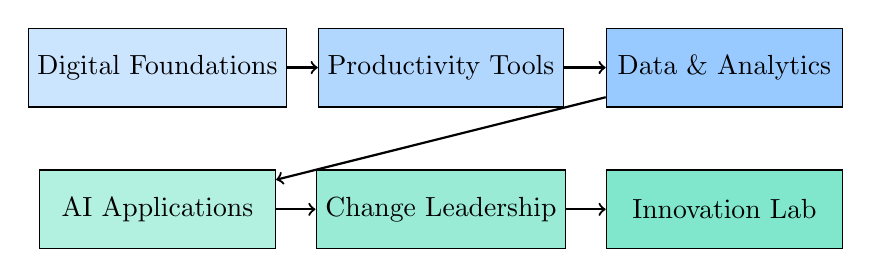
\begin{tikzpicture}[scale=0.9]
            % Module boxes
            \node[draw,fill=dreamblue!20,minimum width=3cm,minimum height=1cm] (m1) at (0,0) {Digital Foundations};
            \node[draw,fill=dreamblue!30,minimum width=3cm,minimum height=1cm] (m2) at (4,0) {Productivity Tools};
            \node[draw,fill=dreamblue!40,minimum width=3cm,minimum height=1cm] (m3) at (8,0) {Data \& Analytics};
            \node[draw,fill=dreamgreen!30,minimum width=3cm,minimum height=1cm] (m4) at (0,-2) {AI Applications};
            \node[draw,fill=dreamgreen!40,minimum width=3cm,minimum height=1cm] (m5) at (4,-2) {Change Leadership};
            \node[draw,fill=dreamgreen!50,minimum width=3cm,minimum height=1cm] (m6) at (8,-2) {Innovation Lab};
            
            % Arrows
            \draw[->,thick] (m1) -- (m2);
            \draw[->,thick] (m2) -- (m3);
            \draw[->,thick] (m3) -- (m4);
            \draw[->,thick] (m4) -- (m5);
            \draw[->,thick] (m5) -- (m6);
        \end{tikzpicture}
    \end{center}
    
    \vspace{1em}
    \begin{columns}[T]
        \column{0.5\textwidth}
        \textbf{Foundation Phase (Months 1-2)}
        \begin{itemize}
            \item Essential digital skills baseline
            \item Productivity quick wins
            \item Data literacy fundamentals
        \end{itemize}
        
        \column{0.5\textwidth}
        \textbf{Transformation Phase (Months 3-6)}
        \begin{itemize}
            \item AI tools implementation
            \item Culture change activation
            \item Service redesign projects
        \end{itemize}
    \end{columns}
    
    \note{Show clear progression and practical outcomes at each stage}
\end{frame}

% Slide 6: ROI Calculator
\begin{frame}{Your Return on Investment}
    \begin{center}
        \textbf{\Large ROI Calculator - Mid-Size Council Example}
    \end{center}
    
    \begin{columns}[T]
        \column{0.5\textwidth}
        \textbf{Investment}
        \begin{itemize}
            \item Programme cost: \highlight{£50,000}
            \item Staff time (20 people × 8 days): £24,000
            \item \textbf{Total investment: £74,000}
        \end{itemize}
        
        \vspace{1em}
        \textbf{Payback Period}
        \begin{center}
            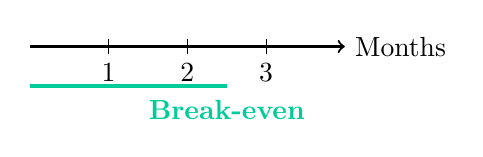
\begin{tikzpicture}
                \draw[thick,->] (0,0) -- (4,0) node[right] {Months};
                \foreach \x in {1,2,3} {
                    \draw (\x,0.1) -- (\x,-0.1) node[below] {\x};
                }
                \draw[dreamgreen,ultra thick] (0,-0.5) -- (2.5,-0.5);
                \node[dreamgreen] at (2.5,-0.8) {\textbf{Break-even}};
            \end{tikzpicture}
        \end{center}
        
        \column{0.5\textwidth}
        \textbf{Annual Benefits}
        \begin{itemize}
            \item Time saved: 2hrs/person/day
            \item = 9,600 hours/year
            \item = \highlight{£288,000} value
            \item Process improvements: £50,000
            \item Reduced errors: £30,000
            \item \textbf{Total benefits: £368,000}
        \end{itemize}
        
        \vspace{1em}
        \centering
        \Large
        \highlight{397\% ROI in Year 1}
    \end{columns}
    
    \note{Make the financial case crystal clear with specific, believable numbers}
\end{frame}

% Slide 7: Case Study Framework
\begin{frame}{Success Story: Salford City Council}
    \begin{columns}[T]
        \column{0.4\textwidth}
        \textbf{The Challenge}
        \begin{itemize}
            \item 3,000+ staff
            \item Legacy systems
            \item Low digital adoption
            \item Budget pressures
        \end{itemize}
        
        \vspace{1em}
        \textbf{The Solution}
        \begin{itemize}
            \item 3-month programme
            \item 25 key staff trained
            \item Focus on quick wins
            \item Peer mentoring activated
        \end{itemize}
        
        \column{0.6\textwidth}
        \textbf{The Results (6 months)}
        
        \begin{center}
            \begin{tikzpicture}
                \begin{axis}[
                    ybar,
                    width=\textwidth,
                    height=0.5\textheight,
                    ylabel={Improvement (\%)},
                    symbolic x coords={Productivity,Satisfaction,Efficiency,Innovation},
                    xtick=data,
                    nodes near coords,
                    ymin=0,ymax=50,
                    bar width=0.8cm,
                    fill=dreamgreen,
                    ]
                    \addplot coordinates {
                        (Productivity,42)
                        (Satisfaction,38)
                        (Efficiency,45)
                        (Innovation,35)
                    };
                \end{axis}
            \end{tikzpicture}
        \end{center}
        
        \vspace{0.5em}
        \textit{"DreamLab transformed how we work. The ROI was evident within weeks." - Sarah Johnson, Director of Digital}
    \end{columns}
    
    \note{Use specific examples and testimonials to build credibility}
\end{frame}

% Slide 8: Implementation Timeline
\begin{frame}{Your Journey to AI Excellence}
    \begin{center}
        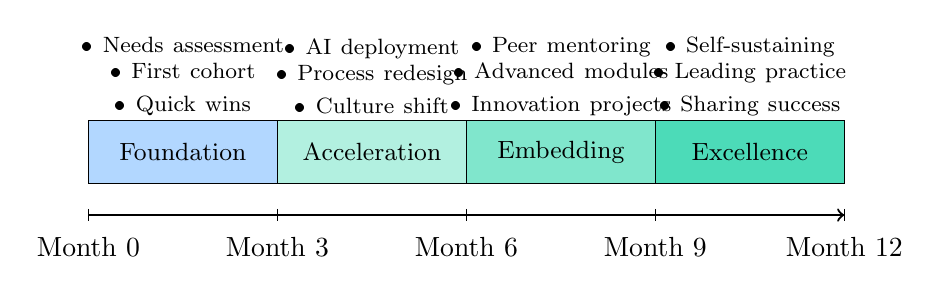
\begin{tikzpicture}[scale=0.8]
            % Timeline
            \draw[thick,->] (0,0) -- (12,0) node[right] {};
            
            % Months
            \foreach \x in {0,3,6,9,12} {
                \draw (\x,0.1) -- (\x,-0.1);
                \node at (\x,-0.5) {Month \x};
            }
            
            % Phase 1
            \draw[fill=dreamblue!30] (0,0.5) rectangle (3,1.5);
            \node at (1.5,1) {\small Foundation};
            \node[text width=3cm,align=center] at (1.5,2.2) {\footnotesize
                • Needs assessment\\
                • First cohort\\
                • Quick wins
            };
            
            % Phase 2
            \draw[fill=dreamgreen!30] (3,0.5) rectangle (6,1.5);
            \node at (4.5,1) {\small Acceleration};
            \node[text width=3cm,align=center] at (4.5,2.2) {\footnotesize
                • AI deployment\\
                • Process redesign\\
                • Culture shift
            };
            
            % Phase 3
            \draw[fill=dreamgreen!50] (6,0.5) rectangle (9,1.5);
            \node at (7.5,1) {\small Embedding};
            \node[text width=3cm,align=center] at (7.5,2.2) {\footnotesize
                • Peer mentoring\\
                • Advanced modules\\
                • Innovation projects
            };
            
            % Phase 4
            \draw[fill=dreamgreen!70] (9,0.5) rectangle (12,1.5);
            \node at (10.5,1) {\small Excellence};
            \node[text width=3cm,align=center] at (10.5,2.2) {\footnotesize
                • Self-sustaining\\
                • Leading practice\\
                • Sharing success
            };
        \end{tikzpicture}
    \end{center}
    
    \vspace{1em}
    \textbf{Support Throughout:}
    \begin{itemize}
        \item Monthly check-ins with your success manager
        \item 24/7 online resource library
        \item Peer council network access
        \item Quarterly best practice workshops
    \end{itemize}
    
    \note{Show clear path to success with ongoing support}
\end{frame}

% Slide 9: Pricing Tiers
\begin{frame}{Investment Options}
    \begin{center}
        \textbf{\Large Choose Your Transformation Path}
    \end{center}
    
    \begin{columns}[T]
        \column{0.33\textwidth}
        \centering
        \textbf{Essential}\\
        \highlight{£15,000 - £25,000}\\
        \vspace{0.5em}
        \begin{itemize}
            \item 3 core modules
            \item Up to 10 staff
            \item Shared cohorts
            \item Online resources
            \item \benefit{Perfect for small councils}
        </end{itemize}
        
        \column{0.33\textwidth}
        \centering
        \textbf{Professional}\\
        \highlight{£30,000 - £60,000}\\
        \vspace{0.5em}
        \begin{itemize}
            \item Full 6 modules
            \item Up to 20 staff
            \item Dedicated cohort
            \item Customisation
            \item \benefit{Ideal for most councils}
        \end{itemize}
        
        \column{0.33\textwidth}
        \centering
        \textbf{Enterprise}\\
        \highlight{£75,000 - £100,000}\\
        \vspace{0.5em}
        \begin{itemize}
            \item All modules + retreat
            \item 30+ staff
            \item Multiple cohorts
            \item Bespoke content
            \item \benefit{For transformation leaders}
        \end{itemize}
    \end{columns}
    
    \vspace{1em}
    \centering
    \textbf{All packages include:}\\
    \faCheckCircle{} Expert instructors
    \faCheckCircle{} CPD certification
    \faCheckCircle{} ROI tracking
    \faCheckCircle{} 12-month support
    
    \note{Clear pricing with obvious value at each tier}
\end{frame}

% Slide 10: Objection Handling
\begin{frame}{Common Concerns Addressed}
    \begin{columns}[T]
        \column{0.5\textwidth}
        \textbf{"We don't have budget"}
        \begin{itemize}
            \item ROI in 2.5 months
            \item Grant funding available
            \item Payment plans offered
            \item Start small, scale up
        \end{itemize}
        
        \vspace{1em}
        \textbf{"Staff don't have time"}
        \begin{itemize}
            \item Saves 2 hours/day after training
            \item Flexible scheduling
            \item Bite-sized modules
            \item Immediate application
        \end{itemize}
        
        \column{0.5\textwidth}
        \textbf{"We've tried training before"}
        \begin{itemize}
            \item This is different - practical focus
            \item Public sector specialists
            \item Ongoing support included
            \item Measurable outcomes
        \end{itemize}
        
        \vspace{1em}
        \textbf{"Our systems are too old"}
        \begin{itemize}
            \item Work with what you have
            \item No IT overhaul needed
            \item Cloud tools included
            \item Future-ready skills
        </invoke>
    \end{columns}
    
    \note{Address objections head-on with confidence}
\end{frame}

% Slide 11: Why DreamLab?
\begin{frame}{Why Choose DreamLab?}
    \begin{columns}[T]
        \column{0.5\textwidth}
        \textbf{Our Unique Advantages}
        \begin{itemize}
            \item \highlight{Only} AI training designed for councils
            \item \highlight{40+} expert practitioners
            \item \highlight{100\%} focus on practical application
            \item \highlight{95\%} participant satisfaction
            \item \highlight{Local} presence in Manchester
        \end{itemize}
        
        \column{0.5\textwidth}
        \textbf{What Makes Us Different}
        \begin{itemize}
            \item We understand council culture
            \item We measure real outcomes
            \item We provide ongoing support
            \item We celebrate your success
            \item We're invested in your region
        \end{itemize}
    \end{columns}
    
    \vspace{1em}
    \begin{center}
        \Large
        \highlight{Join the councils leading the AI revolution}
    \end{center}
    
    \begin{center}
        \includegraphics[width=0.6\textwidth]{client-logos.png}
        % Note: This would show logos of pilot councils
    \end{center}
    
    \note{Build confidence in choosing DreamLab over alternatives}
\end{frame}

% Slide 12: Next Steps
\begin{frame}{Start Your Transformation Journey Today}
    \begin{center}
        \Large
        \textbf{3 Simple Steps to Get Started}
    \end{center}
    
    \vspace{1em}
    \begin{columns}[T]
        \column{0.33\textwidth}
        \centering
        \textbf{\highlight{1. Discovery Call}}\\
        \vspace{0.5em}
        \faPhone\\
        \vspace{0.5em}
        30-minute consultation\\
        Understand your needs\\
        No obligation
        
        \column{0.33\textwidth}
        \centering
        \textbf{\highlight{2. Proposal}}\\
        \vspace{0.5em}
        \faFileAlt\\
        \vspace{0.5em}
        Tailored programme\\
        Clear pricing\\
        ROI projections
        
        \column{0.33\textwidth}
        \centering
        \textbf{\highlight{3. Launch}}\\
        \vspace{0.5em}
        \faRocket\\
        \vspace{0.5em}
        Start within 4 weeks\\
        First results in days\\
        Transform your council
    \end{columns}
    
    \vspace{2em}
    \begin{center}
        \Large
        \highlight{Book your discovery call today}\\
        \vspace{0.5em}
        \normalsize
        \faPhone{} 0161 XXX XXXX\\
        \faEnvelope{} councils@dreamlab.co.uk\\
        \faGlobe{} dreamlab.co.uk/councils
    \end{center}
    
    \note{Clear call to action with easy next steps}
\end{frame}

% Appendix
\appendix

% Detailed Module Breakdown
\begin{frame}{Appendix: Module Details}
    \small
    \begin{tabular}{p{3cm}|p{4cm}|p{3cm}}
        \toprule
        \textbf{Module} & \textbf{What You'll Learn} & \textbf{Outcomes} \\
        \midrule
        Digital Foundations & Cloud concepts, collaboration tools, security basics & 30\% faster daily tasks \\
        Advanced Productivity & Automation, AI assistants, workflow design & 2+ hours saved daily \\
        Data-Driven Decisions & Analytics, dashboards, predictive insights & Evidence-based policies \\
        AI Applications & ChatGPT, computer vision, process automation & 40\% efficiency gains \\
        Change Leadership & Digital champions, culture shift, adoption & 80\% staff engagement \\
        Service Innovation & Design thinking, emerging tech, citizen experience & New service models \\
        \bottomrule
    </end{tabular}
    
    \vspace{1em}
    \textbf{Delivery Options:}
    \begin{itemize}
        \item Intensive weeks (full immersion)
        \item Monthly sessions (gradual transformation)
        \item Hybrid delivery (online + in-person)
        \item Residential retreat (deep dive)
    \end{itemize}
    
    \note{Detailed information available for those wanting specifics}
\end{frame}

% Grant Funding Options
\begin{frame}{Appendix: Funding Opportunities}
    \textbf{Available Grant Schemes}
    \begin{itemize}
        \item \highlight{UK Shared Prosperity Fund} - Skills programmes
        \item \highlight{Innovate UK} - Digital transformation
        \item \highlight{Local Growth Fund} - Productivity improvements
        \item \highlight{Adult Education Budget} - Workforce development
    \end{itemize}
    
    \vspace{1em}
    \textbf{How We Help:}
    \begin{itemize}
        \item Identify suitable funding streams
        \item Support application writing
        \item Provide evidence of impact
        \item Meet funding requirements
    \end{itemize}
    
    \vspace{1em}
    \centering
    \highlight{Many councils access 50-100\% funding for our programme}
    
    \note{Financial barriers can often be overcome with grant funding}
\end{frame}

\end{document}